\documentclass[../Article_Model_Parameters.tex]{subfiles}
\graphicspath{{\subfix{../Figures/}}}
\begin{document}

    A supercritical fluid (SCF) is any substance at a temperature and pressure above its critical point, where distinct liquid and gas phases do not exist, but below the pressure required to compress it into a solid. It can effuse through porous solids like a gas, overcoming the mass transfer limitations that slow liquid transport through such materials. SCF are much superior to gases in their ability to dissolve materials like liquids or solids. Also, near the critical point, small changes in pressure or temperature result in large changes in density, allowing many properties of a supercritical fluid to be "fine-tuned". By changing the pressure and temperature of the fluid, the properties can be "tuned" to be more liquid-like or more gas-like. 
    
    %Carbon dioxide above its critical point attains a supercritical state and exhibits certain peculiar properties such as higher density as a liquid but with a lower viscosity comparable to a gas. The supercritical carbon dioxide (S-CO2) has a range of engineering applications. 

    The properties of a fluid can be divided into two kinds, equilibrium properties and transport properties. The equation of state can be used accurately to predict the equilibrium properties, such as density, enthalpy, vapor pressure, fugacity and fugacity coefficient, vapor liquid equilibrium, and all kinds of excess properties.
    
    The thermodynamic properties of supercritical $CO_2$ such as density, local speed of sound and specific heat capacity vary significantly for slight change in temperature and pressure due to real gas effects. Equation of state (EOS) which account these real gas effects is used to calculate the thermodynamic properties. In order to predict this real gas effects, the Peng-Robinson equation of state (P-R EOS) is used to compute properties of $CO_2$. Detail information about Peng-Robinson equation of state can be found in the work of \citet{Peng1976}, \citet{Elliott2011} or \citet{Pratt2001}. The P-R EOS belongs to the specific class of thermodynamic models for modelling the pressure of a gas as a function of temperature and density and can be written as a cubic function of the molar volume (of the density). The P-R EOS is presented by equation \ref{EQ: PR}

    {\footnotesize
        \begin{equation}
            P = \cfrac{RT}{V_m - b} - \cfrac{a\alpha}{V_m^2 + 2bV_m - b^2}
            \label{EQ: PR}
        \end{equation}
    }

    where $a, b, \alpha$ are parameters defined as presented in the appendix.
    
    The properties of the $CO_2$ presented as a function of operating conditions (temperature and pressure) are presented on fig. \ref{fig: SFE_Properties}    
    
    At standard atmospheric pressure and temperature, the $CO_2$ behaves as an ideal gas, and its compressibility factor equals to unity.  However, at high temperature and pressure, the compressibility factor varies from unity, due to real gas effects. As it is presented on Figure \ref{fig: SFE_Properties_Compressibility}, the compressibility factor obtained from the Peng-Robinson equation of state varies strongly depending on the operating conditions. The compressibility factor can be obtained by given temperature and pressure by solving the polynomial form of the P-R EOS given by equation \ref{EQ: PR_polynomial}.

    {\footnotesize
    \begin{equation}
        Z^3 - (1-B)Z^2+(A-2B-3B^2)Z -(AB-B^2-B^3) = 0
        \label{EQ: PR_polynomial}
    \end{equation}
    }

    where $A$ and $B$ are parameters as defined in the appendix (\ref{CH: Thermodynamic_details}). The roots of the polynomial can be found iteratively or by Cardano formula. Depends on the operating conditions, one or two roots can be found. In one-phase region the fluid can be describe as gas, liquid or super-critical. In the two-phase region the gas-liquid mixture is present. The biggest root is assigned to the gas phase and smallest root corresponds to the liquid phase.

    The real gas effects are also visible on the density plot presented on the Figure \ref{fig: SFE_Properties_Density}. The density can change significantly depends on the operating conditions. 
    By analysing the compressibility and density plots more it can be noticed that very near to the critical point, the fluid can neither be called a liquid nor a gas and has a unique combination of gas-like and liquid-like properties. 

    The Figure \ref{fig: SFE_Properties_CP} show behaviour of the heat capacity of a supercritical fluid at constant pressure ($C_p$). The details of the calculations can be found in the appendix. In contrary to the density which varies monotonically, the specific heat shows very high levels in a narrow region. In the subcritical region, the phase transition is associated with an effective spike in the heat capacity (i.e., the latent heat). Approaching the critical point, the latent heat falls to zero but this is accompanied by a gradual rise in heat capacity in the pure phases near phase transition. At the critical point, the latent heat is zero but the heat capacity shows a diverging singularity. Beyond the critical point, there is no divergence, but rather a smooth peak in the heat capacity; the highest point of this peak identifies the Widom line (as discussed by \citet{Simeoni2010} and \citet{Banuti2019}).

    In order to calculate thermodynamic properties from a real gas, the departure function for that property with respect to the chosen equation of state has to be evaluated. As presented by \citet{Elliott2011}, the departure function for any thermodynamic property of a real gas is defined as the difference in the value of that property determined from the chosen real gas equation of state and the value of the same property for an ideal gas under the same conditions of temperature and pressure. %(10.1007/s10494-017-9872-4)

	%{\color{blue}The Peng-Robinson equation of state is used to describe the thermodynamics of the fluid phase. The thermal properties of the pseudo-homogeneous phase are assumed to vary along the extractor, though always remaining equal to the corresponding mean values between the fluid and solid phase. }
			
	%In the process model, properties of the supercritical fluid such as the density ${\color{orange}\rho} ({\color{blue}T}(t,z),{\color{red}P}(t))$, the specific heat ${\color{orange}C_p}({\color{blue}T}(t,z),{\color{red}P}(t))$, the thermal conductivity ${\color{orange}k^T}({\color{blue}T}(t,z),{\color{red}P}(t))$, or the viscosity ${\color{orange}\eta}({\color{blue}T}(t,z),{\color{red}P}(t))$ are calculated based on the local temperatures along the fixed bed and the pressure. The Peng-Robinson equation of state is used to find values of a ${\color{orange}\rho} ({\color{blue}T}(t,z),{\color{red}P}(t))$ and ${\color{orange}C_p}({\color{blue}T}(t,z),{\color{red}P}(t))$.
			
		\begin{figure*}[H]
			\begin{subfigure}[b]{0.95\textwidth}
				\centering
				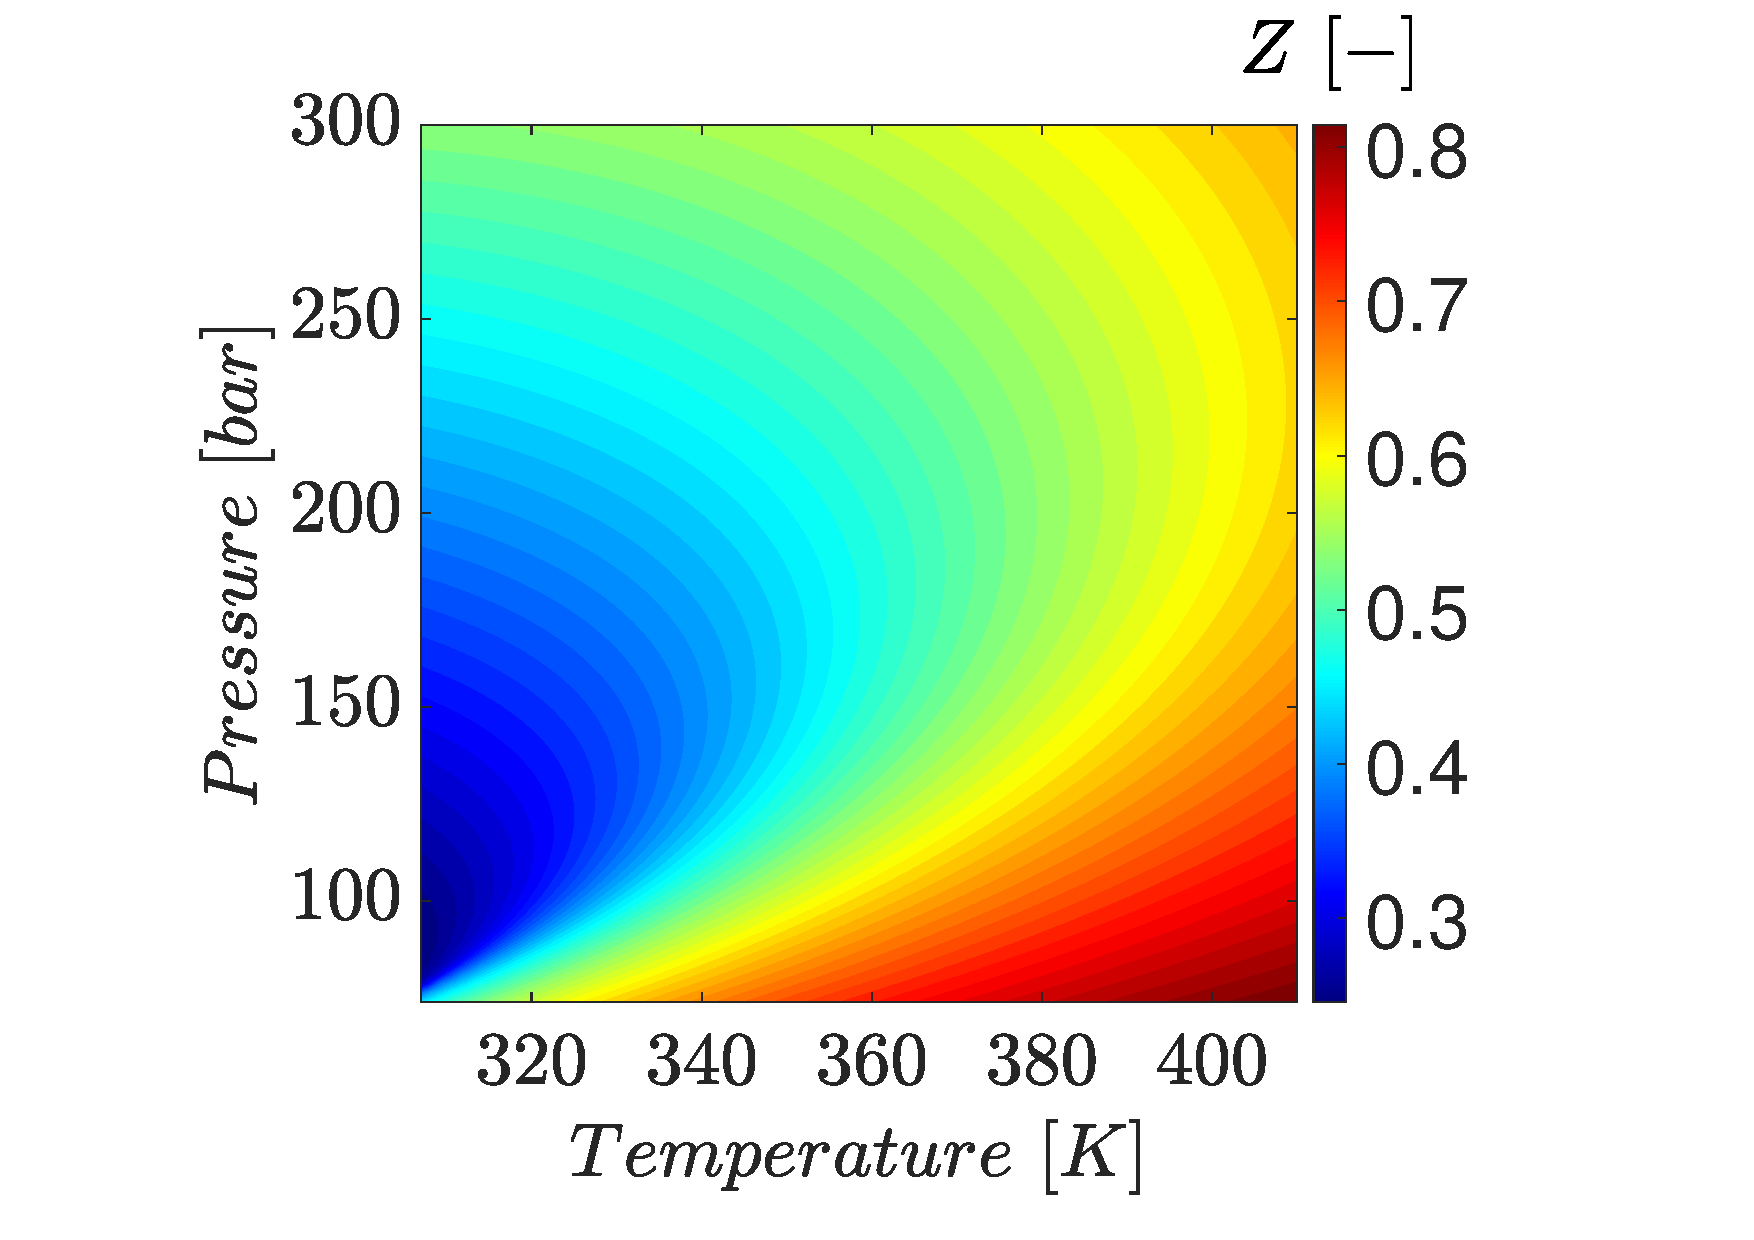
\includegraphics[trim = 2.9cm 7cm 3cm 7cm,clip,width=\textwidth]{Figures/Compressibility.pdf}	
				\caption{The compressibility factor based on the Peng-Robinson equation of state}
                \label{fig: SFE_Properties_Compressibility}
			\end{subfigure}
			\hfill
			\begin{subfigure}[b]{0.95\textwidth}
				\centering
				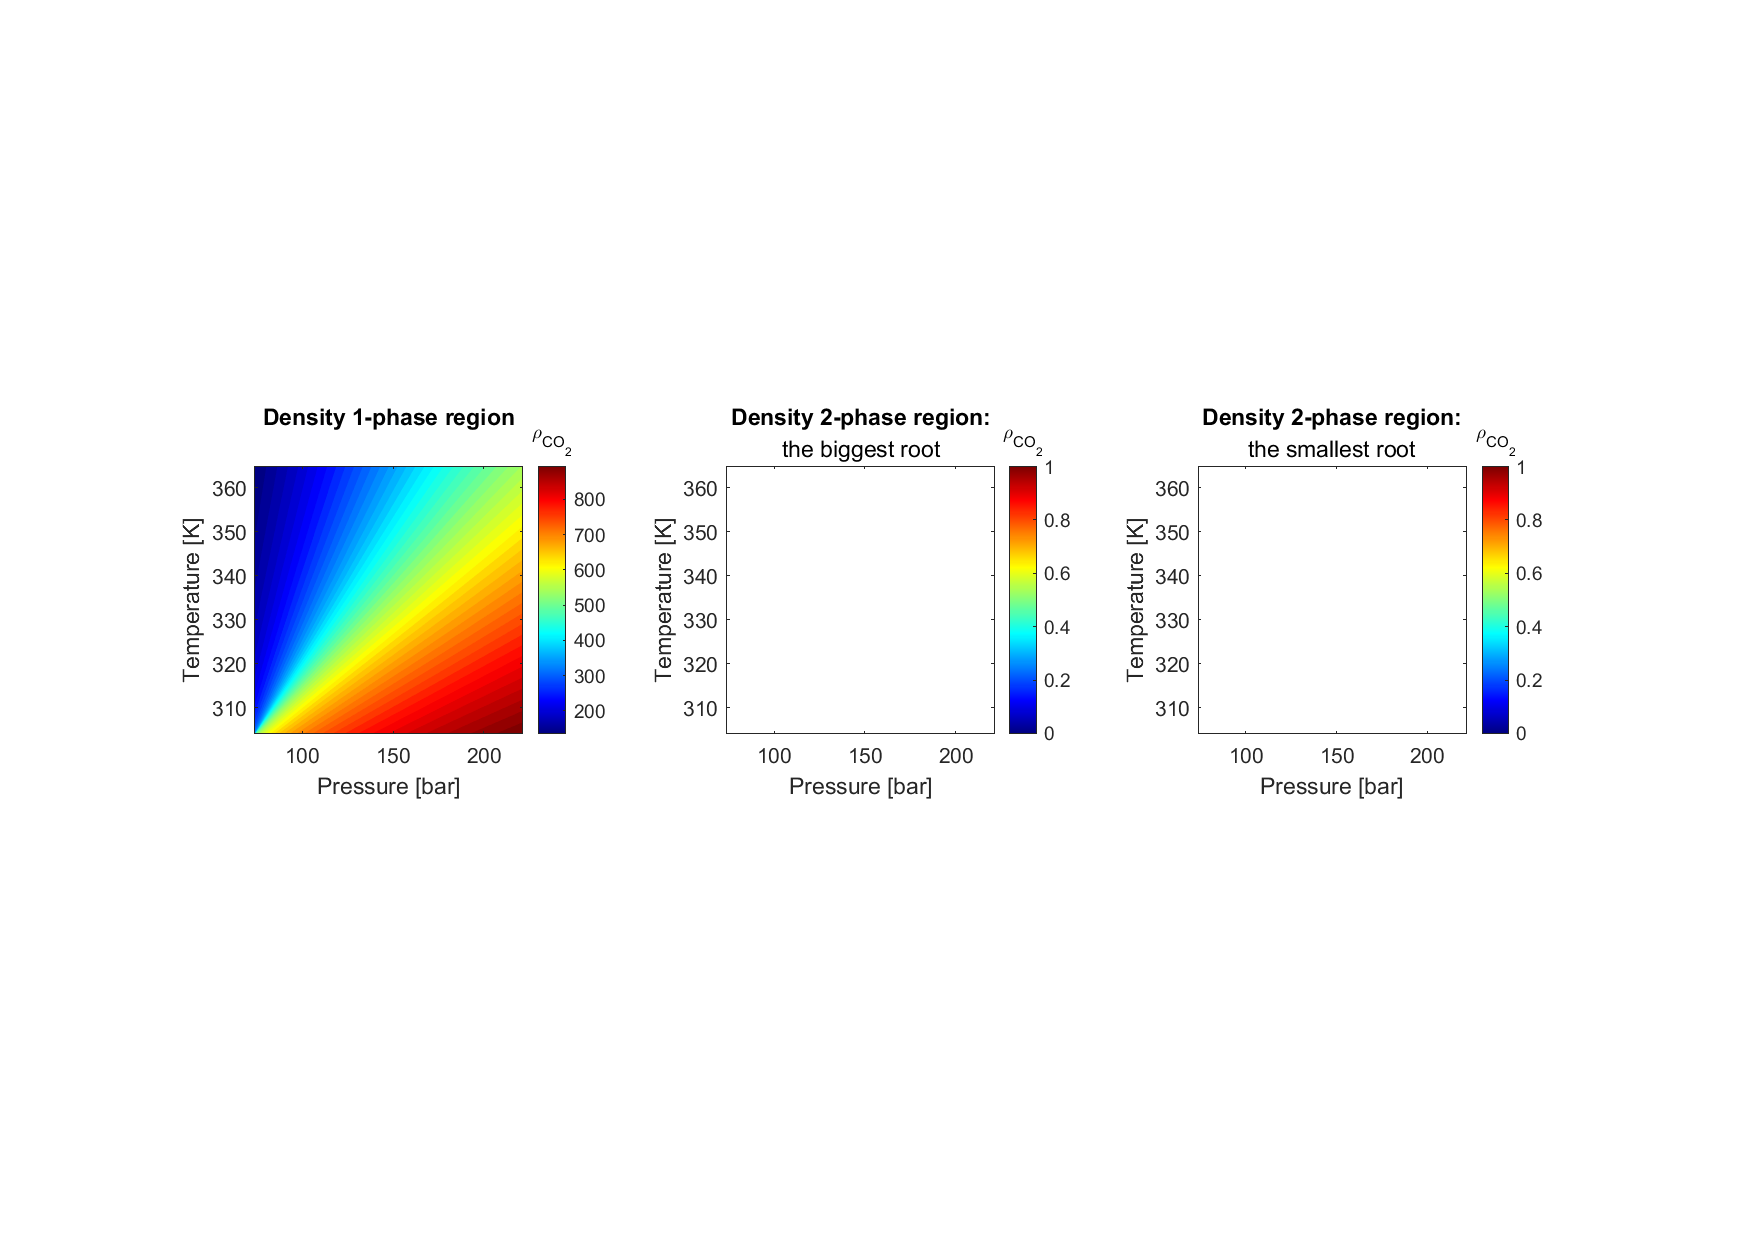
\includegraphics[trim = 2.9cm 7cm 3cm 7cm,clip,width=\textwidth]{Figures/RHO.pdf}	
				\caption{The fluid density based on the Peng-Robinson equation of state}
                \label{fig: SFE_Properties_Density}
			\end{subfigure}
			\hfill
			\begin{subfigure}[b]{0.95\textwidth}
				\centering
				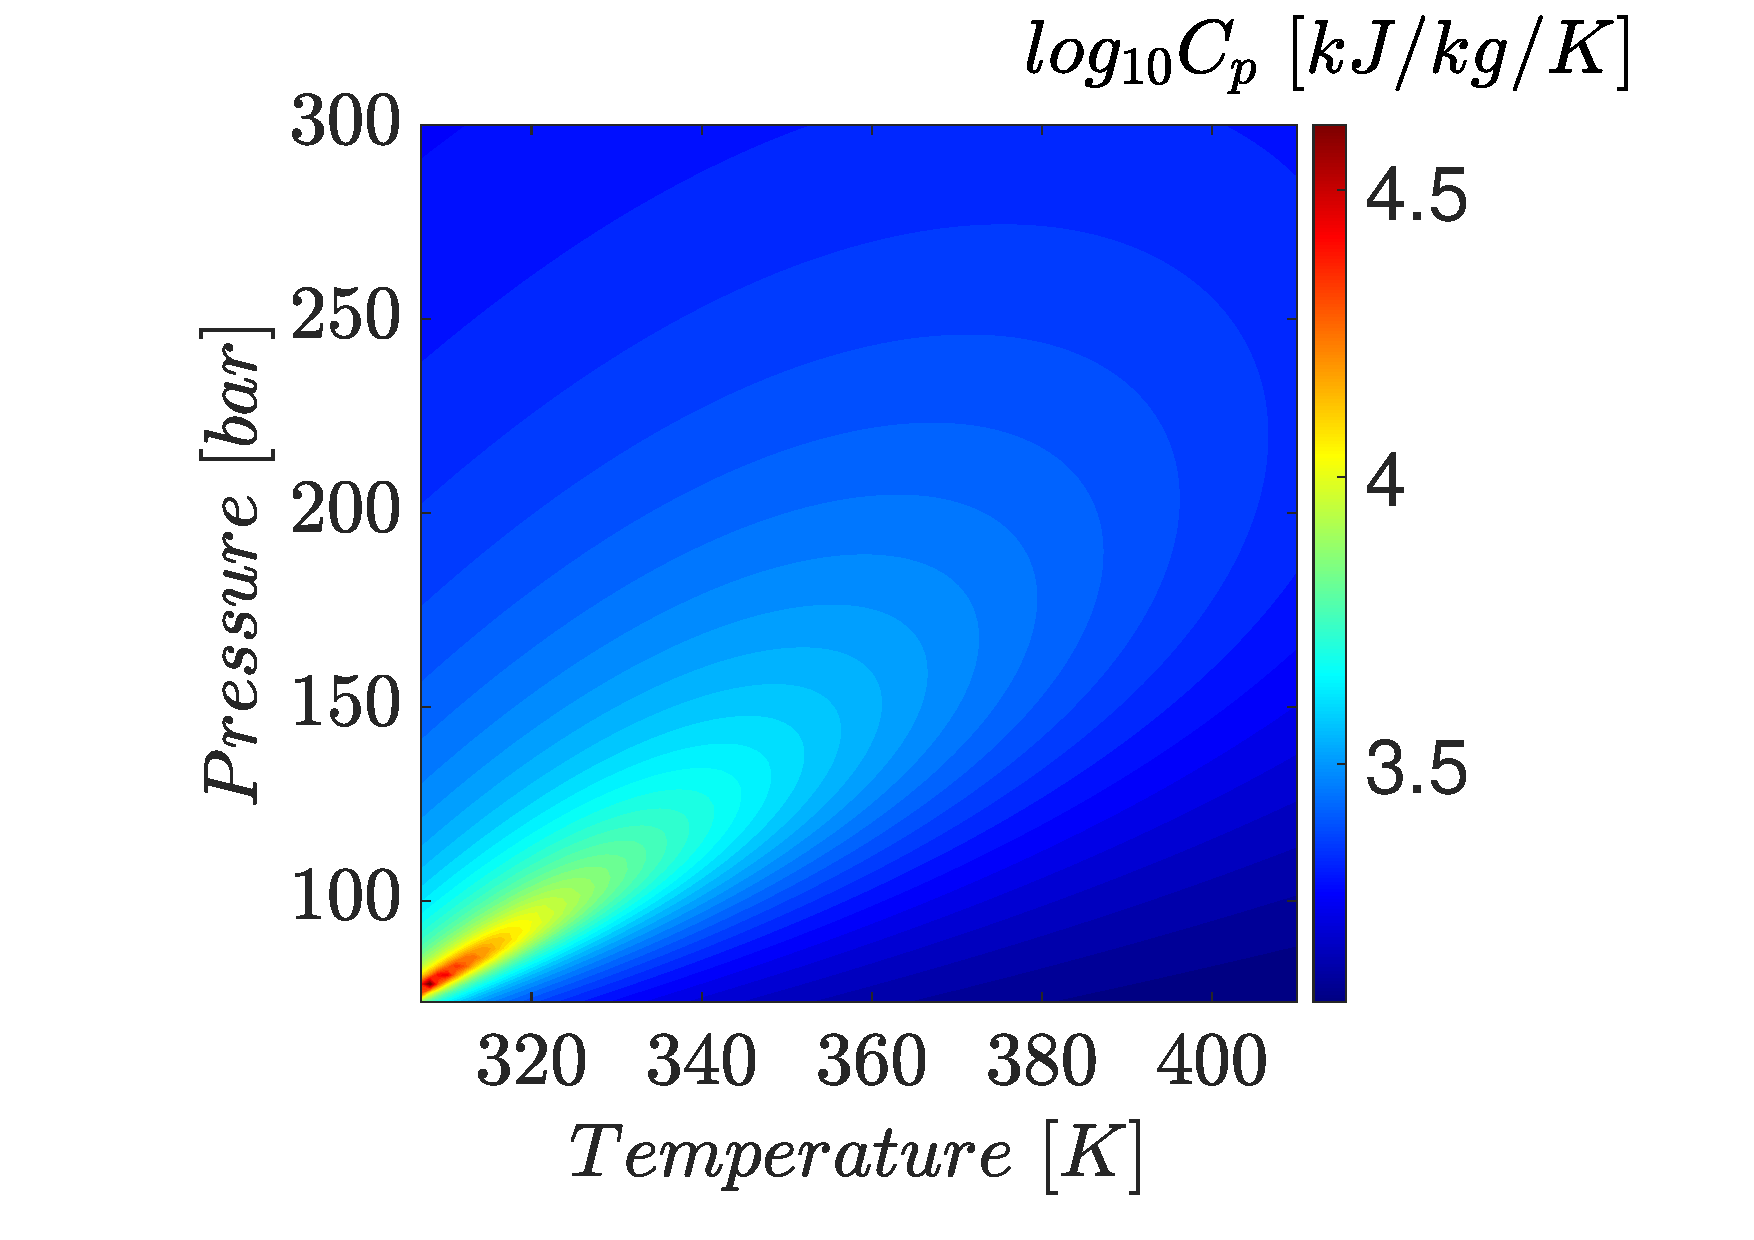
\includegraphics[trim = 2.9cm 7cm 3.cm 7cm,clip,width=\textwidth]{Figures/CP.pdf}	
				\caption{The specific heat of the $CO_2$ based on the Peng-Robinson equation of state}
                \label{fig: SFE_Properties_CP}
			\end{subfigure}
			\caption{Properties of $CO_2$ based on the equation of state}
			\label{fig: SFE_Properties}
		\end{figure*}    

        On the other hand, transport properties (viscosity and conductivity) are also important quantities required in engineering design for production, fluid transportation, and processing. According to \citet{Sheng1989}, there is no satisfactory theory of transport properties of real dense gases and liquids. The main difficulties in the study of transport properties are twofold: one is the inherent difficulties involved in accurate measurements, and the other is the complexity involved in theoretical treatments. Therefore, the generally used correlations of transport coefficient are either empirical or based on some theoretical foundation. Enskog (\todo[fancyline]{Add ref}) developed a popular theory for the transport properties of dense gas based on the distribution function. However, the Enskog theory was proposed for rigid spherical molecules. For real gases, some modification is needed. Following the Enskog theory, many correlations have been proposed in the form of the reduced density and reduced temperature. The correlations of \citet{Fenghour1998} and \citet{Laesecke2017} implemented and compared as presented on Figure \ref{fig: SFE_Properties_mu}. The viscosity formulation proposed by NIST consists of four contributions: (i) for the limit of zero density, (ii) for the initial density dependence, (iii) for the residual viscosity, and (iv) for the singularity of the viscosity at the critical point. The NIST correlation covers temperatures from 100 to 2000 $K$ for gaseous $CO_2$ and from 220 to 700 $K$ with pressures along the melting line up to 8000 $MPa$ for compressed and supercritical liquid states. 
			
		%The inter-particle diffusion coefficient ${\color{orange}D^M_e}(\allowbreak{\color{blue}T}(t,z),{\color{red}P}(t),{\color{red}F}(t))$ is calculated from the empirical correlation, as the function of the Reynolds number ${\color{orange}R_e}({\color{blue}T}(t,z),{\color{red}P}(t),\allowbreak{\color{red}F}(t))$ and the Peclet's number ${\color{orange}P_e}({\color{blue}T}(t,z),\allowbreak{\color{red}P}(t),{\color{red}F}(t))$.
		%The values of the internal diffusion ${\color{orange}D_i} ({\color{blue}T}(t,z))$ and the partition coefficient ${\color{orange}k_m} ({\color{blue}T}(t,z))$ come from the laboratory experiments. The expressions and the detailed information of the parameter fitting can be found in the appendix.

        \begin{figure*}[H]
			\centering
			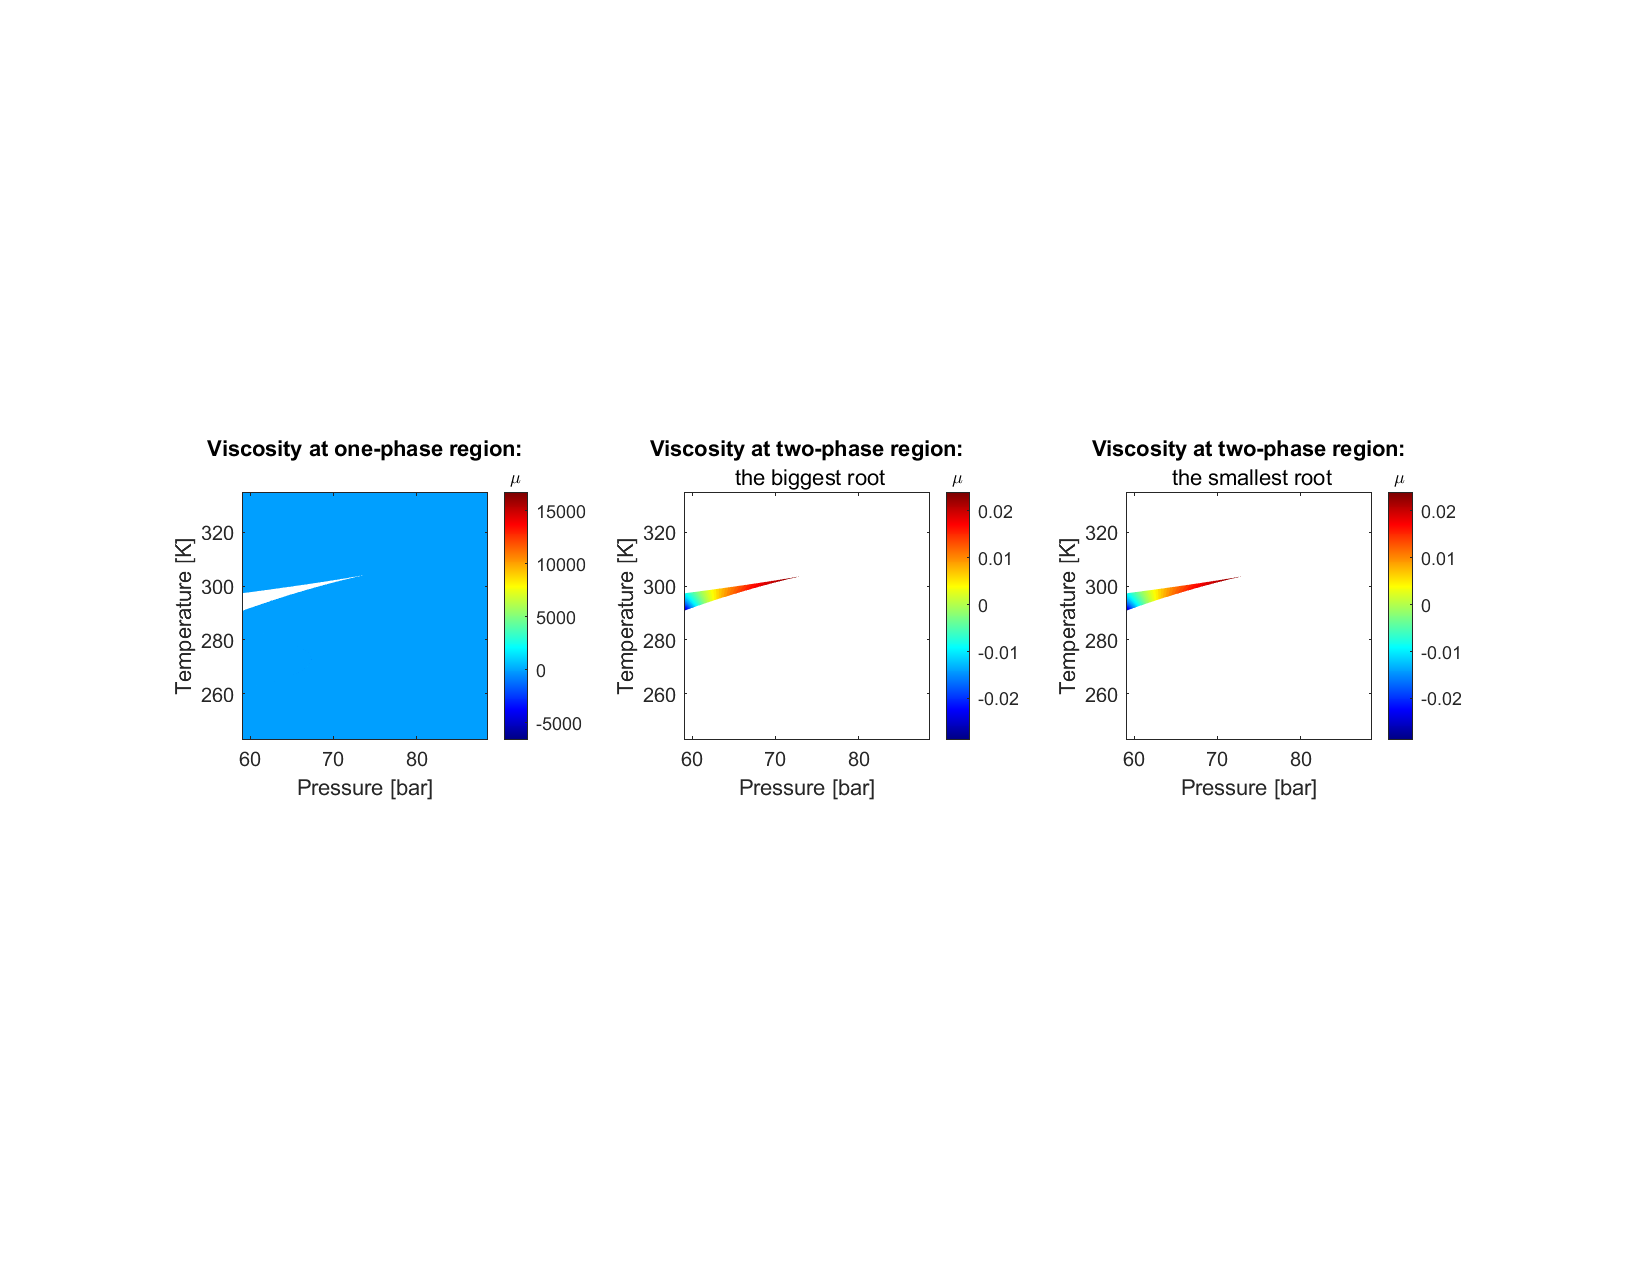
\includegraphics[trim = 1.5cm 11.5cm 2.5cm 10.0cm,clip,width=\textwidth]{Figures/MU.pdf}	
			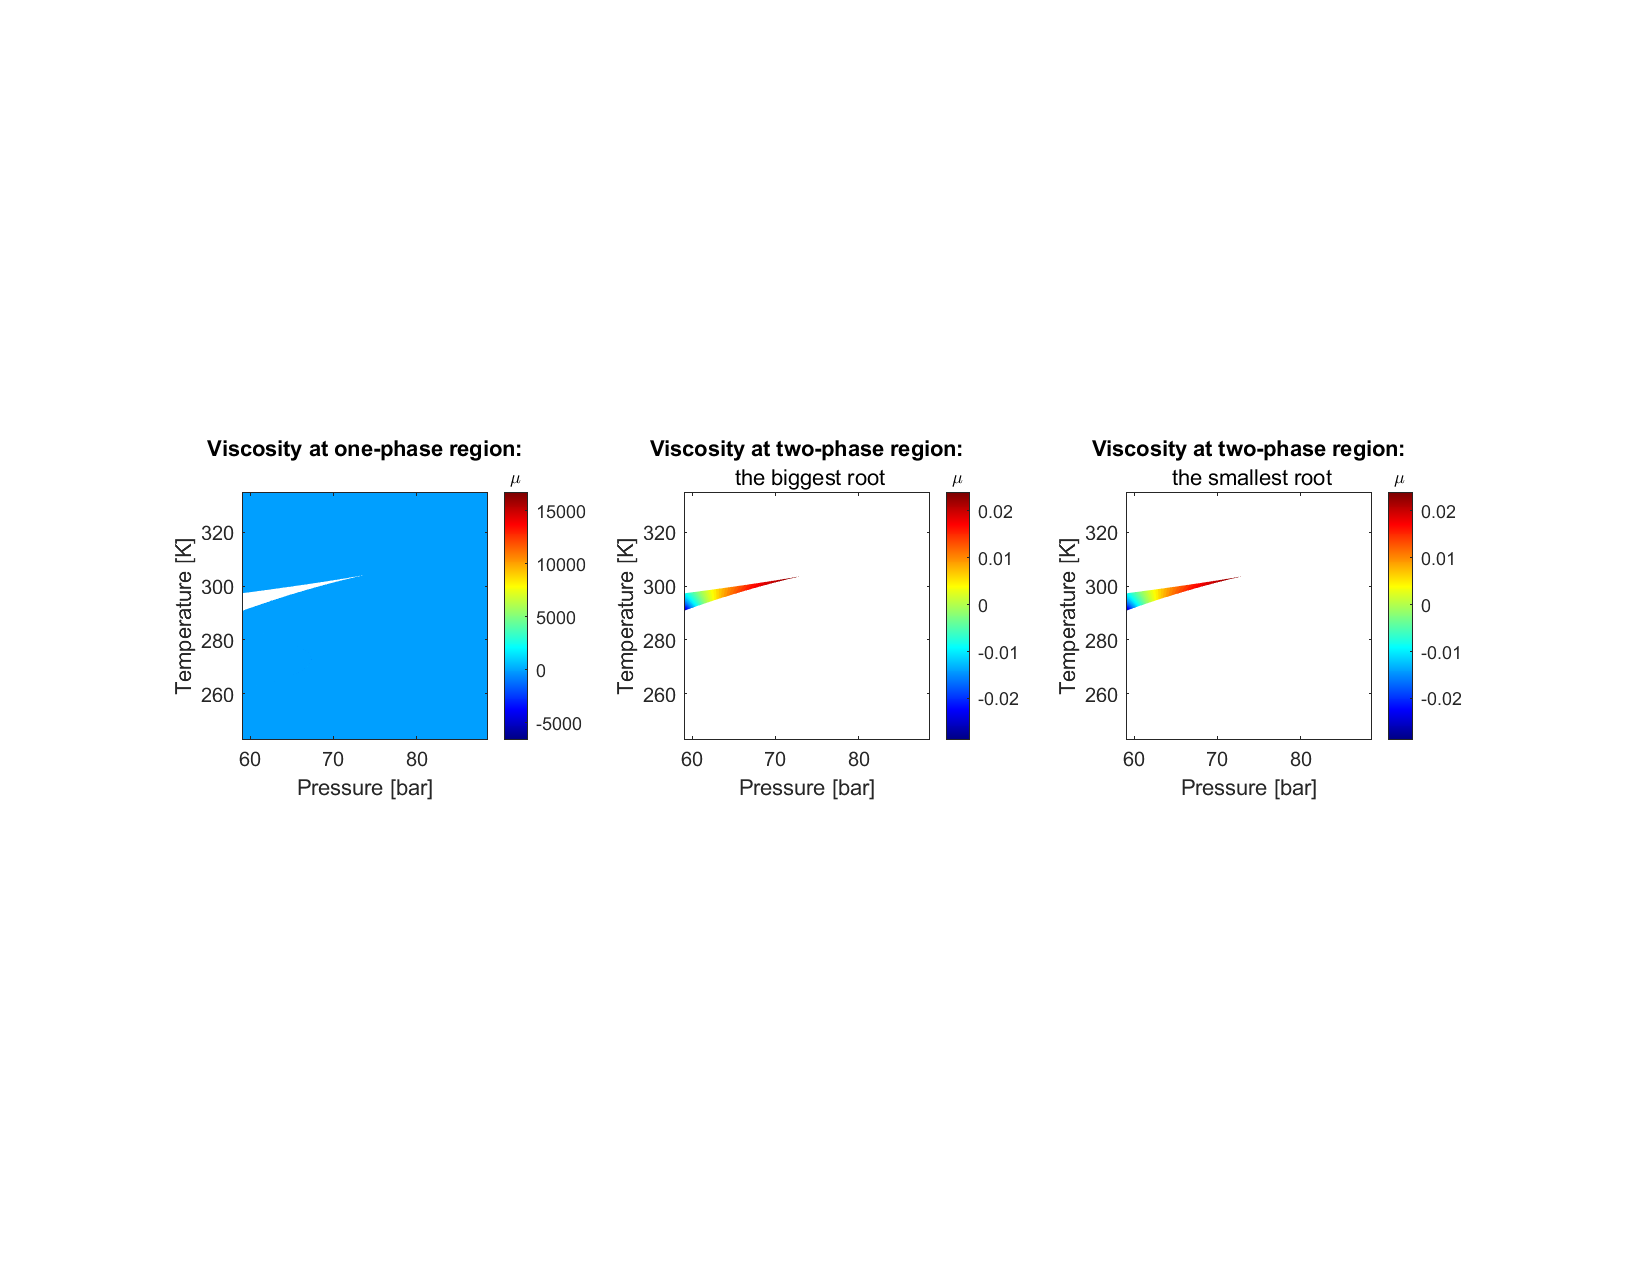
\includegraphics[trim = 1.5cm 4.0cm 2.5cm 19.0cm,clip,width=\textwidth]{Figures/MU.pdf}	
			\caption{Viscosity obtained based on different correlations } 
            \label{fig: SFE_Properties_mu}
		\end{figure*} 
			
        Similarly, several correlations for thermal conductivity of $CO_2$ were compared on Figure \ref{fig: SFE_Properties_kt}. The presented figures are focused around critical point, where the singularity is present. Similarities between specific heat and the thermal conductivity can be observed. The NIST correlation (\citet{Huber2016}) captures the singular behaviour of thermal conductivity around the critical point. The correlations are applicable for the temperature range from the triple point to 1100 $K$ and pressures up to 200 $MPa$. 

        \begin{figure*}[H]
			\centering
			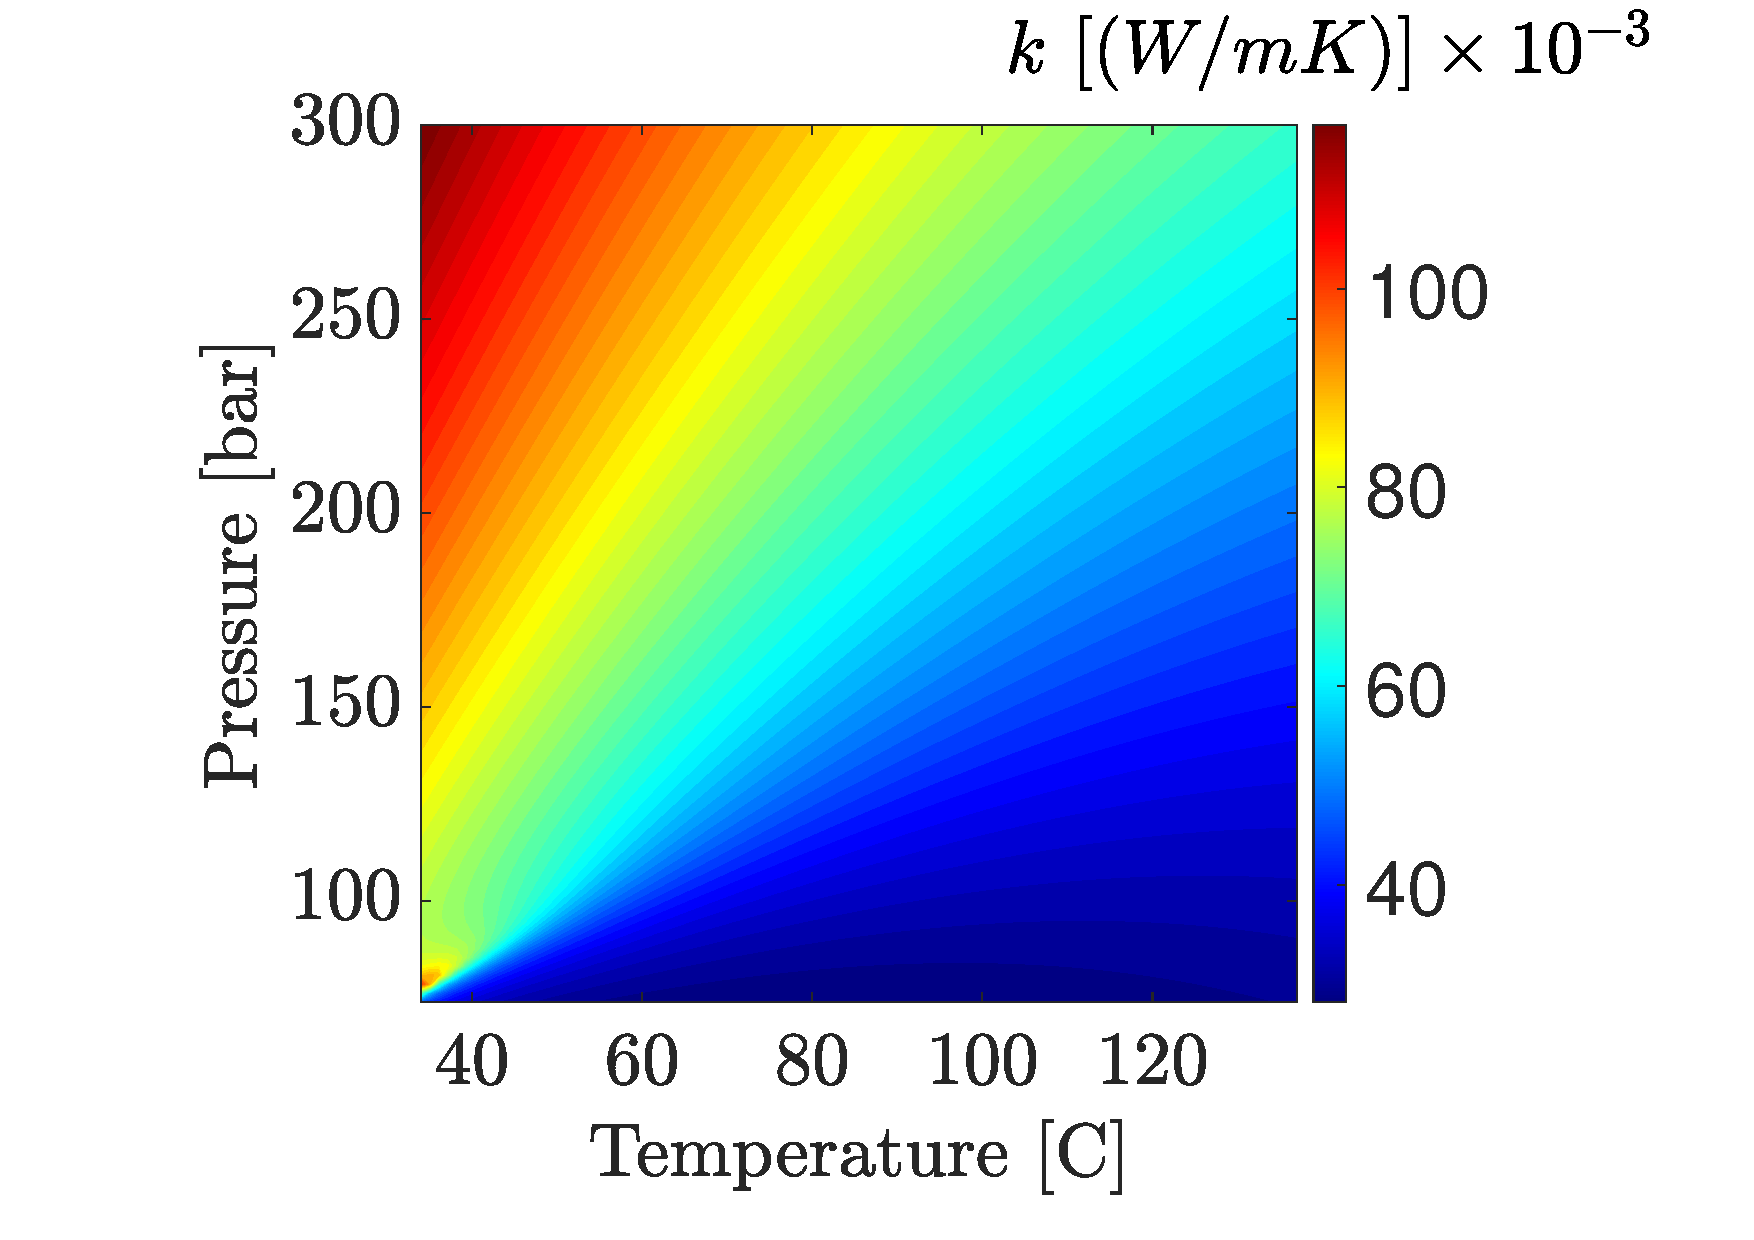
\includegraphics[trim = 1.5cm 2.5cm 1.5cm 2.0cm,clip,width=0.95\textwidth]{Figures/KT.pdf}	
			\caption{Thermal conductivity obtained based on different correlations }
            \label{fig: SFE_Properties_kt}
		\end{figure*} 

\end{document}